
\section{Information Flow Theory} 
The following sections give a brief introduction to the general notion of \emph{security} in regards to the concept of information in computational systems.
Building upon this, we then focus specifically on the key concepts of non-interference and declassification as they relate to the notion of information flow.
\subsection{Security models and policies}
Many modern computational systems will at some point have to handle certain kinds of information, which must never be accessible to an \emph{unauthorized} entity.
A popular description for a system, which keeps its information from leaking to the outside or any unintended entity/process can be found in the term of a  \emph{secure} system.
In this context, ``security'' or ``secure information flow'' means, that "no unauthorized flow of information is possible" \cite{lattice_model_security}.

While such a general definition may be relatively easy to arrive at, actually \emph{enforcing} the necessary constraints on the numerous information pipelines and flows within even a single program is often no easy task at all. 
In order to properly define which information may flow in what way within a part of a program or between programs, a common approach is to specify the individual components, between which a flow of information may occur and consequently assigning certain security \emph{levels} to these individual constituents. This approach can for example be found in \cite{lattice_model_security} by \citeauthor{lattice_model_security}, in which the concept of \emph{security classes} \(SC\) is introduced. These classes can then be bound to any information receptacles or ``objects'' in order to denote their respective security clearance.
\todo{This chapter is way too short at the moment.}
\todo{Mention, that the lattice model is very widespread and fundamental. Tie into this later aswell. (Public/Private can be seen as a binary lattice model.)}
\subsection{Non-interference and Declassification}
\label{ref:Declass_and_Inter}
An important concept in terms of secure systems that can be operated by multiple users either simultaneously or sequentially, is the concept of \emph{non-interference}.
\begin{quotation}
    One group of users, using a certain set of commands, is noninterfering with another group of users if what the first group does with those commands has no effect on what the second group of users can see
\end{quotation}

To explain this concept in terms of our problem domain of PGP servers, let us assume running instance of HAGRID which is publicly accessible. Let us further assume that there are two users \(u1\) and \(u2\) that are interacting with the server at the same time. Additionally, each user holds a certain set of keys:


\(
    u1 := \begin{cases}
        k1 = \text{Key(id1,id2)} \\
        k2 = \text{Key(id3,id4)}
    \end{cases}
    \) and \, \(
    u2 := \begin{cases}
        k3 = \text{Key(id5,id6)} \\
        k4 = \text{Key(id7,id8)}
    \end{cases}
    \)

Based on this, we can image the following, highly simplified interaction between the two users and HAGRID
\begin{figure}[H]
    \label{fig:example}
    \centering
    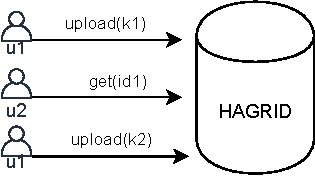
\includegraphics{images/non_interference.pdf}
    \caption{A non-interfering interaction}
\end{figure}

The second call of \(u2\) in this sequence is a key request for identity \(id1\) which belongs to the previously uploaded key \(k1\). Yet, because the identity had not been verified when \(u2\) issued its key request, the resulting response will be empty. That means, that the actions of \(u1\) hat no effect \emph{at all} on the experience of \(u2\). 
As a matter of fact, based on the interactions with HAGRID alone, \(u2\) has no way of identifying whether there even \emph{is} another user currently interacting with the same system. 
In contrast to that, let us assume that this sequence of interactions is continued in the following way: 
\begin{figure}[H]
    \label{fig:example}
    \centering
    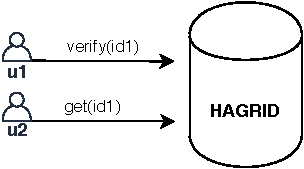
\includegraphics{images/interfering.pdf}
    \caption{The interaction has become interfering}
\end{figure}

The second \(get\) request now yields a different response as before. Instead of an empty response, \(u2\) now receives a key with an identity. This change in behaviour was caused by \(u1\) issuing a verification for \(id1\). Therefore, the actions of \(u1\) were able to influence the sequence of interactions between \(u2\) and HAGRID, which causes this interaction to no longer be \emph{non-interfering}. \\ \\

Given this definition of non-interference, it can be trivially concluded that a strict enforcement of this principle would render most information systems practically unusable.
Instead, what we need is a formal mechanism to determine the circumstances under which the release of classified information is permissible. As mentioned in \cite{declass_dim_prin}, one key concern of any system that permits the declassification of private information is, whether that release is actually \emph{safe}. That means, whether the introduction of additional declassification policies would allow an attacker to obtain more information from the given system than intended by its designers.
\\
This safety concern has given rise to a multitude of different approaches, which aim at formally verifying the correct flow and release of information. Some of these approaches will be briefly laid out in chapters \ref{sec:related_work} and \emph{REF TODO}.
\\ \\
However, the central approach of this thesis will specifically focus on the testing of \emph{dynamic} information flow policies.

\textbf{TODO: Why is this too strict? Examples.}
\textbf{TODO: How does declassification work?}
% \textbf{TODO: Tie this into previous chapter, Flow from HIGH to LOW is declassification in a way.}
\todo{Quote Security Policies and Security Models for their definition of non-interference}

\newpage
